\documentclass[a4paper,12pt,openany,oneside]{article}
\usepackage[a4paper,top=2cm,bottom=2cm,left=2cm,right=3cm]{geometry}
\usepackage[utf8]{inputenc}
\usepackage{pgfplots}
\pgfplotsset{compat=1.12}
\usepgfplotslibrary{fillbetween}
\usetikzlibrary{patterns}
\usepackage[hidelinks]{hyperref}

\title{Complex Numbers}
\author{Lorenzo Bonanni}
\date{October 2021}



\begin{document}
\maketitle
Source: \href{https://youtu.be/5PcpBw5Hbwo}{\color{blue}\textit{Complex number fundamentals | Lockdown math ep. 3}}

\newpage
\section{Assumptions}
\parbox{400pt} {
\begin{itemize}
    \item There's a number i so that $i^2=-1$
    \item i stays on a different number line that's perpendicular to Real Numbers
    \begin{tikzpicture}[scale=0.80]
        \begin{axis}[
            xmin=-3, xmax=3,
            ymin=-3, ymax=3,
            axis lines=middle,
            ytick={2, 1, 0, -1, -2},
            yticklabels={$2i$, $i$, 0, $-i$, $-2i$},
        ] 
        \end{axis}
    \end{tikzpicture}
\end{itemize}
}
\newpage
\section{Operations}
\subsection{Sum}
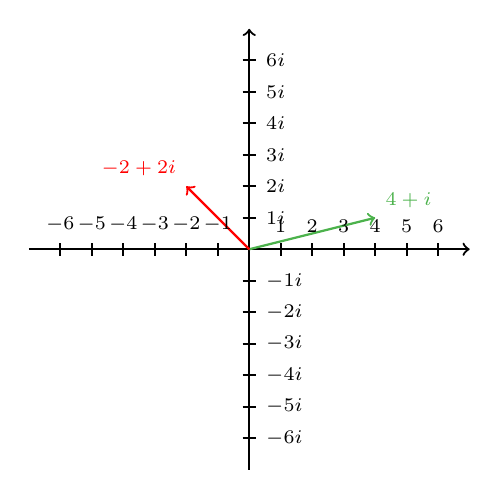
\begin{tikzpicture}[scale=0.40]
    \begin{scope}[thick,font=\scriptsize]
    % Axes:
    % Are simply drawn using line with the `->` option to make them arrows:
    % The main labels of the axes can be places using `node`s:
    \draw [->] (-7,0) -- (7,0);
    \draw [->] (0,-7) -- (0,7);
    \draw [->, color=green!40!gray] (0,0) -- (4, 1) node [above right] {$4+i$};
    \draw [->, color=red] (0,0) -- (-2, 2) node [above left] {$-2+2i$};
    
    \foreach \n in {-6,...,-1,1,2,...,6}{%
        \draw (\n,-6pt) -- (\n,6pt)   node [above] {$\n$};
        \draw (-6pt,\n) -- (6pt,\n)   node [right] {$\n i$};
    }
    \end{scope}
\end{tikzpicture}
\\
To sum those two vectors $-2+2i$ and $4+i$ we simply divide the imaginary part from the real one and then we sum those single components.\\
\textbf{Real Part:} $(4-2)$\\
\textbf{Imaginary Part:} $(1-2)i$\\
So the \textbf{result} is $2+3i$
\subsection{Multiplication}
Suppose we have the point (3,2) what is the 90° rotation of that point counterclockwise?\\
\\
\begin{minipage}{.2\textwidth}
\begin{tikzpicture}[scale=0.40]
    \begin{scope}[thick,font=\scriptsize]
    % Axes:
    % Are simply drawn using line with the `->` option to make them arrows:
    % The main labels of the axes can be places using `node`s:
    \draw [->] (-7,0) -- (7,0);
    \draw [->] (0,-7) -- (0,7);
    % \draw [->, color=green!40!gray] (0,0) -- (4, 1) node [above right] {$4+i$};
    % \draw [->, color=red] (0,0) -- (-2, 2) node [above left] {$-2+2i$};
    \draw (3,2) node[anchor=south] {\textbullet};
    
    \foreach \n in {-6,...,-1,1,2,...,6}{%
        \draw (\n,-6pt) -- (\n,6pt)   node [above] {$\n$};
        \draw (-6pt,\n) -- (6pt,\n)   node [right] {$\n i$};
    }
    \end{scope}
\end{tikzpicture}
\end{minipage}
\hspace{4cm}% NO SPACE!
\begin{minipage}{.2\textwidth}
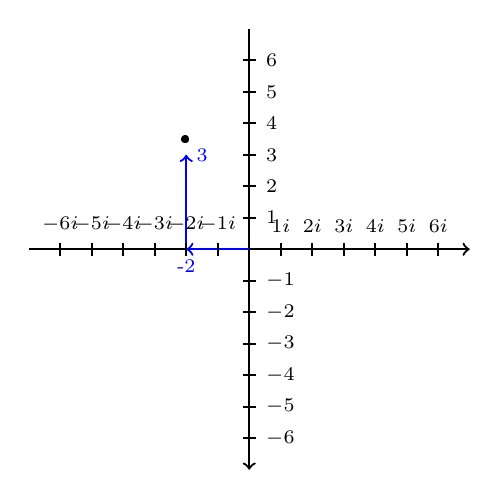
\begin{tikzpicture}[scale=0.40]
    \begin{scope}[thick,font=\scriptsize]
    % Axes:
    % Are simply drawn using line with the `->` option to make them arrows:
    % The main labels of the axes can be places using `node`s:
    \draw [->] (-7,0) -- (7,0);
    \draw [<-] (0,-7) -- (0,7);
    \draw [thick, ->, color=blue] (0,0) -- (-2, 0) node [below] {-2};
    \draw [thick, ->, color=blue] (-2, 0) -- (-2, 3) node [right] {3};;
    % \draw [->, color=red] (0,0) -- (-2, 2) node [above left] {$-2+2i$};
    \draw (-2, 3) node[anchor=south] {\textbullet};
    
    \foreach \n in {-6,...,-1,1,2,...,6}{%
        \draw (\n,-6pt) -- (\n,6pt)   node [above] {$\n i$};
        \draw (-6pt,\n) -- (6pt,\n)   node [right] {$\n$};
    }
    \end{scope}
\end{tikzpicture}
\end{minipage}
\\
To find out let's rotate the Entire plane 90°\\
\begin{minipage}{200pt}
(3,2)-90°CW$\rightarrow$(-2,3)\\
(a,b)-90°$\rightarrow$(-b,a)-90°$\rightarrow$(-a,-b)
\end{minipage}\\
\hspace{30pt}
\begin{center}
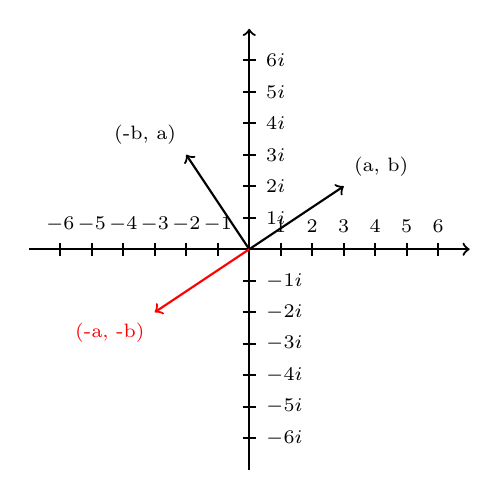
\begin{tikzpicture}[scale=0.40]
    \begin{scope}[thick,font=\scriptsize]
    % Axes:
    \draw [->] (-7,0) -- (7,0);
    \draw [->] (0,-7) -- (0,7);
    % ticks
    \foreach \n in {-6,...,-1,1,2,...,6}{
        \draw (\n,-6pt) -- (\n,6pt)   node [above] {$\n$};
        \draw (-6pt,\n) -- (6pt,\n)   node [right] {$\n i$};
    }
    
    % vectors
    \draw [->, color=black, thick] (0,0) -- (3, 2) node [above right] {(a, b)};
    \draw [->, color=black, thick] (0,0) -- (-2, 3) node [above left] {(-b, a)};
    \draw [->, color=red, thick] (0,0) -- (-3, -2) node [below left] {(-a, -b)};
    \end{scope}
\end{tikzpicture}
\end{center}
\newpage
Lets calculate the following equation $3*(3+2i)$:\\
$3*(3+2i) = 3i+2i^2 = 3i+2*(-1) = -2+3i$\\
As we can see the result is like rotating $3*(3+2i)$ by 90°\\
\subsubsection{3 Facts about Multiplications}
\begin{enumerate}
    \item $z*1=z$
    \item $z*i=Rot90(z)$
    \item $z*(c+di)=c*z+d*(zi)$
\end{enumerate}
Let's solve $(2+i)(2-i)$\\
$(2+i)(2-i) =\\ 2*2+2i-2i-i^2 = \\4+0i-(-1) =\\ 5+0i = 5$
\vspace{10pt}
\\
\textbf{What is the complex number $z$ so that multiplying by $z$ has the effect of rotating 30°, or $\frac{\pi}{6}$ radians, counterclockwise?\\}
$z=cos(\pi/6)+isin(\pi/6)$\\[0.5cm]

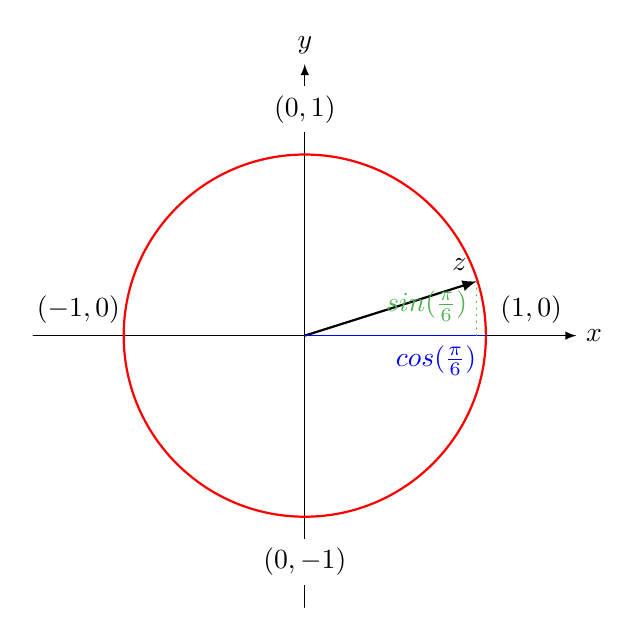
\begin{tikzpicture}[scale=2.3,cap=round,>=latex]
    % draw the coordinates
    \draw[->] (-1.5cm,0cm) -- (1.5cm,0cm) node[right,fill=white] {$x$};
    \draw[->] (0cm,-1.5cm) -- (0cm,1.5cm) node[above,fill=white] {$y$};

    % draw the unit circle
    \draw[thick, color=red] (0cm,0cm) circle(1cm);
    
    % draw the horizontal and vertical coordinates
    % the placement is better this way
    \draw (-1.25cm,0cm) node[above=1pt] {$(-1,0)$}
          (1.25cm,0cm)  node[above=1pt] {$(1,0)$}
          (0cm,-1.25cm) node[fill=white] {$(0,-1)$}
          (0cm,1.25cm)  node[fill=white] {$(0,1)$};
          
    \draw [->, color=black, thick] (0,0) -- (0.95cm, 0.3cm) node [above left]
    {$z$};
    \draw [-, color=blue] (0,0) -- (1cm, 0cm) node [below left]{$cos(\frac{\pi}{6})$};
    \draw [-, color=green!40!gray, dotted] (0.95cm,0) -- (0.95cm, 0.3cm) node [below left]{$sin(\frac{\pi}{6})$};
\end{tikzpicture}
\end{document}
